\chapter{实验验证}


\section{验证指标}
\section{接触验证}
\section{节点分布验证}
\section{小结}

In this section, T-START mobility model is validated on the aspects of node distribution compared with existing mobility models and the real traces. We pick two simple mobility models for comparison: one free space - Random Way Point (RWP) model, the other is constrained model, Shortest Path (SP).  SP mobility model is based on the underlying map of Beijing where vehicles move along the map roads by Dijkstra algorithm to random destinations. Both models take no consideration of the node statuses. All mobility models are implemented on Opportunistic Networking Environment (ONE)\cite{KeranenOtt-155}.

In our simulations, vehicles are deployed in an area of $24,000\times 24,000 m^2$, including fourth ring roads in Beijing.
To evaluate the time feature of T-START, 4 time periods are chosen: in the morning from 6:00:00 to 7:59:59, at noon from 11:00 to 13:00, at afternoon from 17:00 to 19:00 and lat in the evening from 22:00 to 24:00. Accordingly, we extract the real traces at corresponding time period of 21st November 2011.
3000 taxies are randomly selected. 
We need to configure the speed range for RWP and SP mobility model. Those two models will generate a new speed randomly in the speed range. We set the speed range from 0 to twice the average speed for certain time period.
The average speed for RWP and SP are set as $15.83km/h$ for 6:00 to 8:00, $18.43km/h$ for 11:00 to 13:00, $15.25km/h$ for 17:00 to 19:00 and $20.46km/h$ for 22:00 and 24:00. 
Thus, the speed ranges for the four time periods are $[0, 36.86]km/h$, $[0, 36.86]km/h$, $[0, 30.50]km/h$ and $[0, 40.802]km/h$.

\begin{figure}[!t]
\centering
\subfigure[Real Trace]{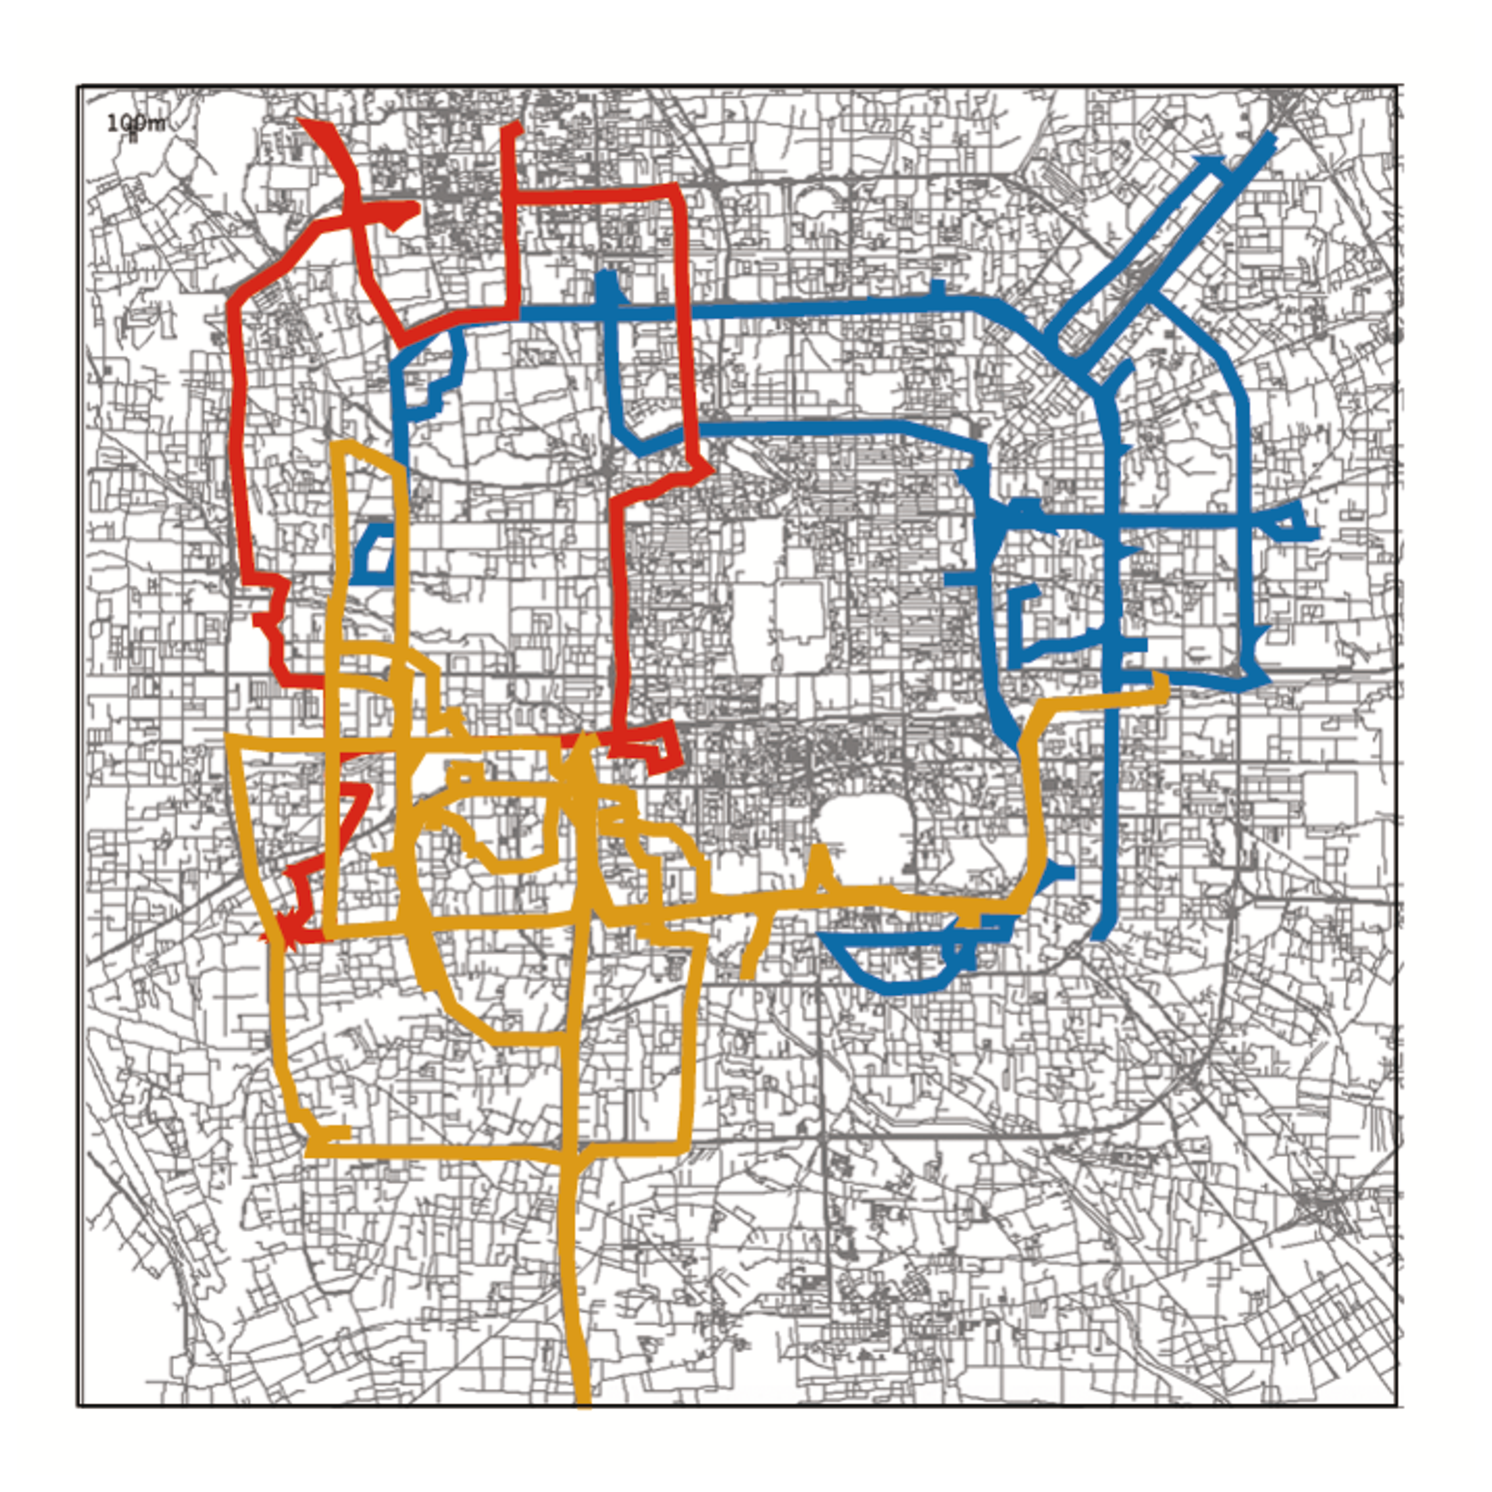
\includegraphics[width=0.24\textwidth]{figures/evalue/sample/real_traces.eps}}
\subfigure[T-START]{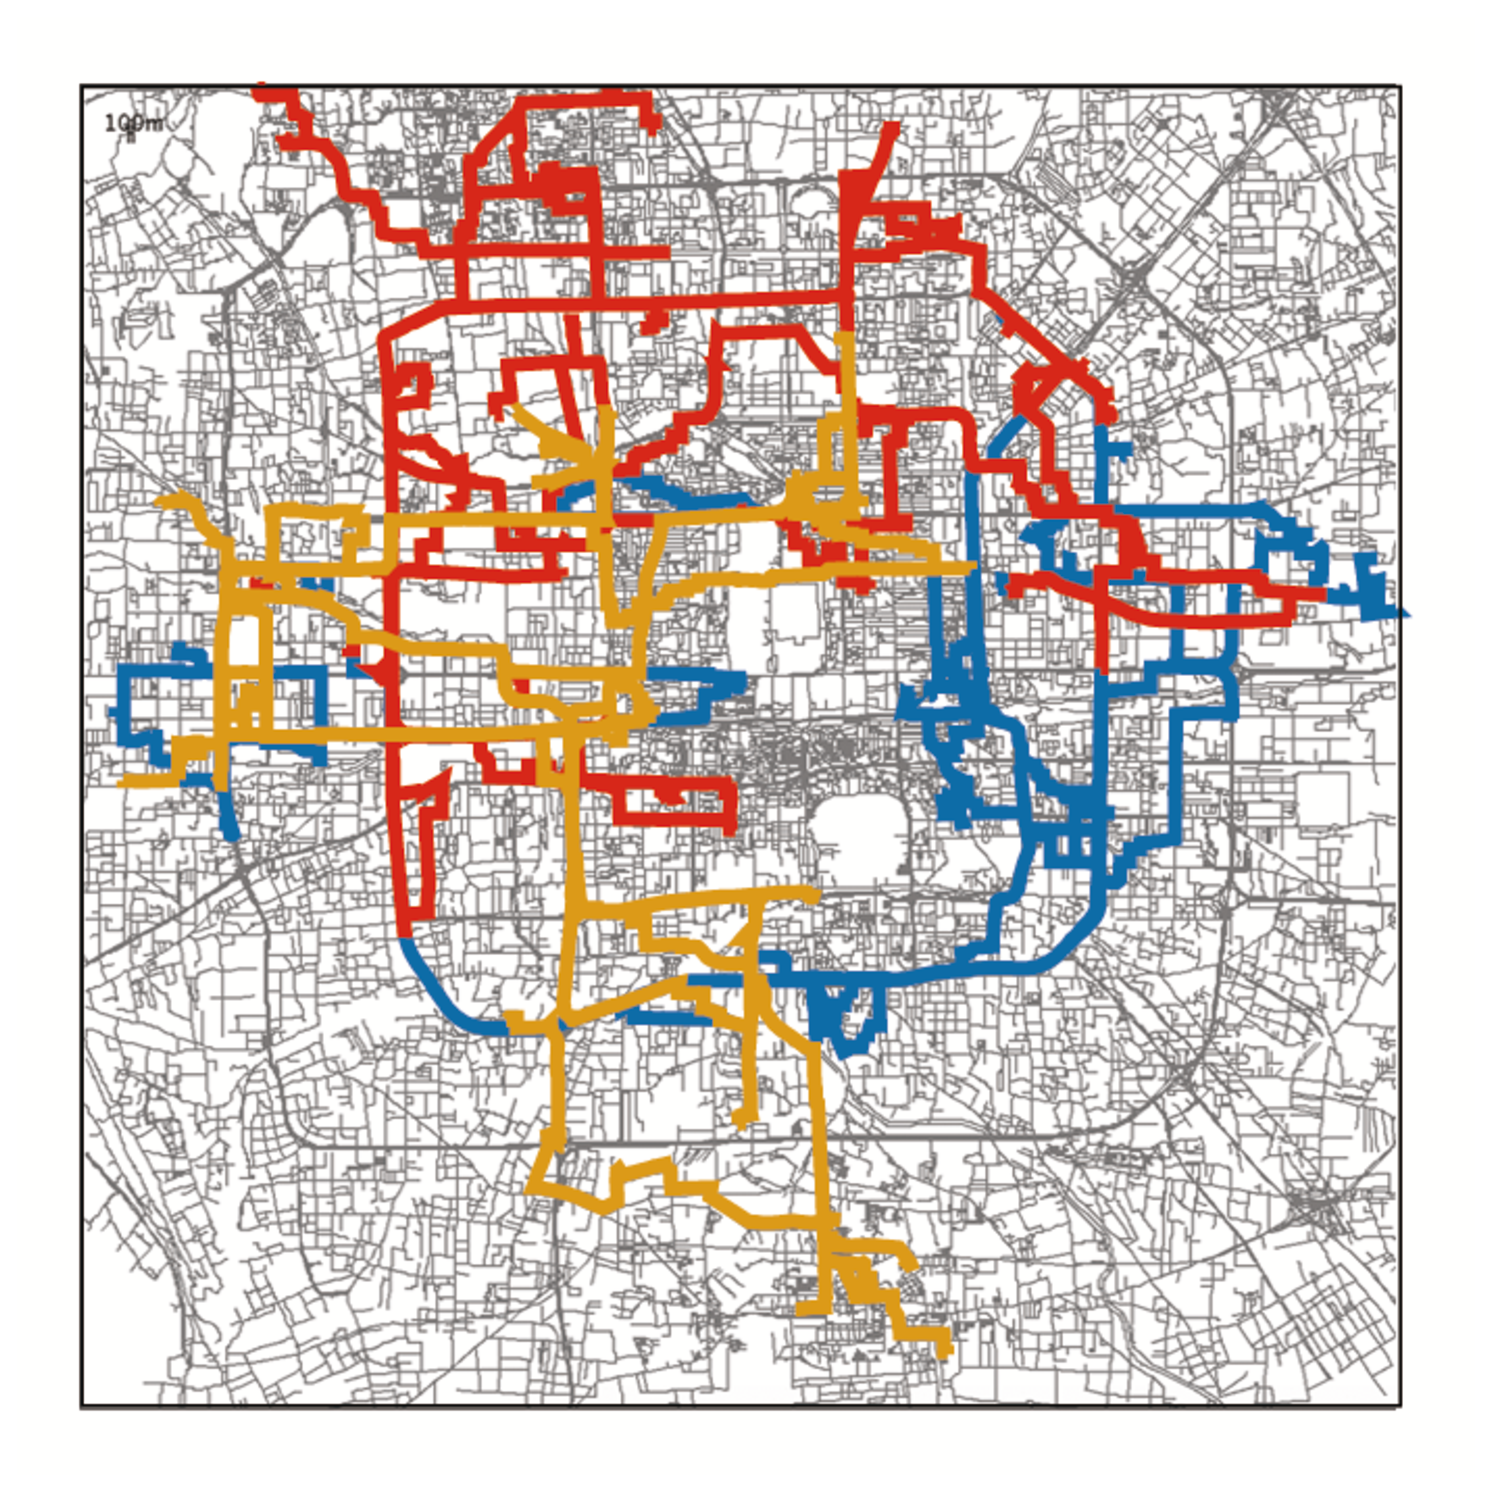
\includegraphics[width=0.24\textwidth]{figures/evalue/sample/start_traces.eps}}
\subfigure[SP]{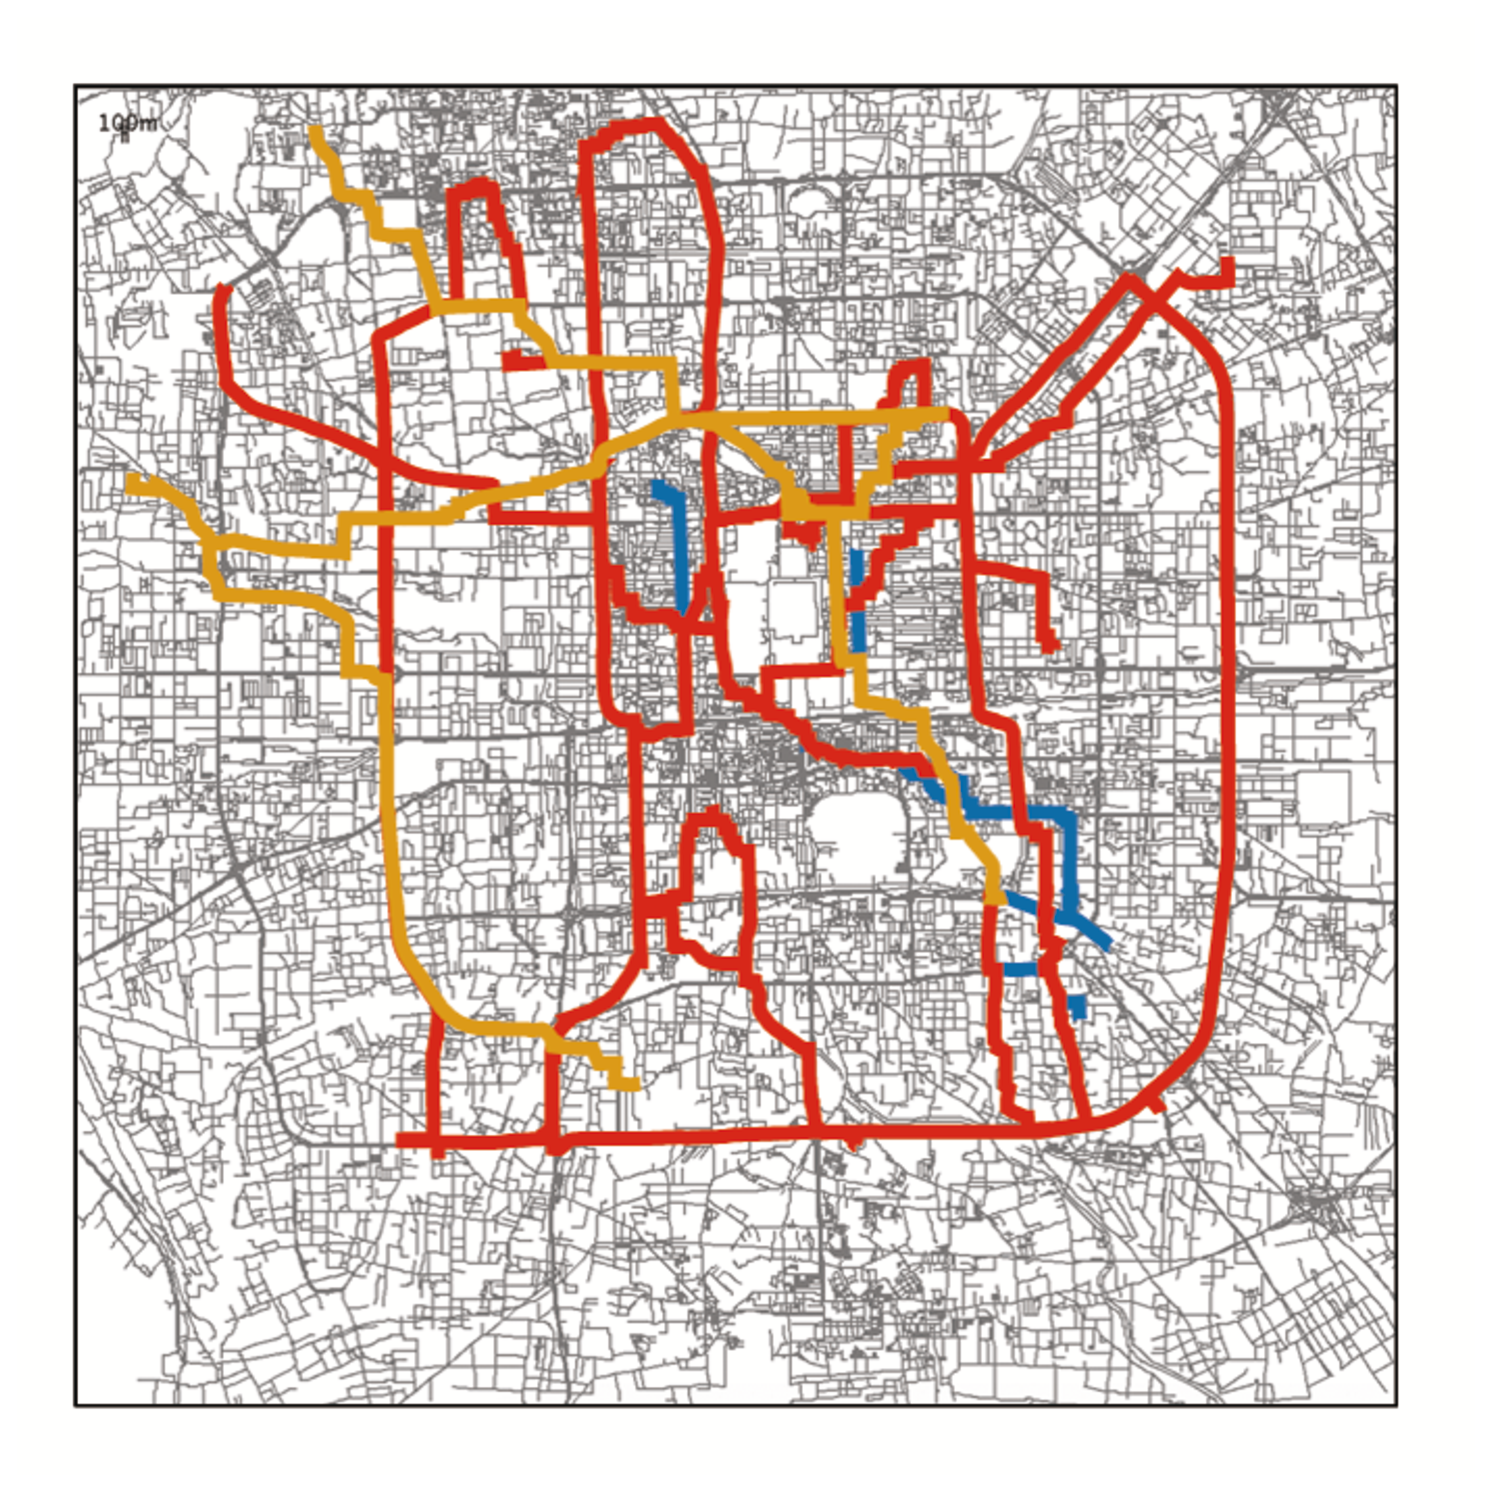
\includegraphics[width=0.24\textwidth]{figures/evalue/sample/sp_traces.eps}}
\subfigure[RWP]{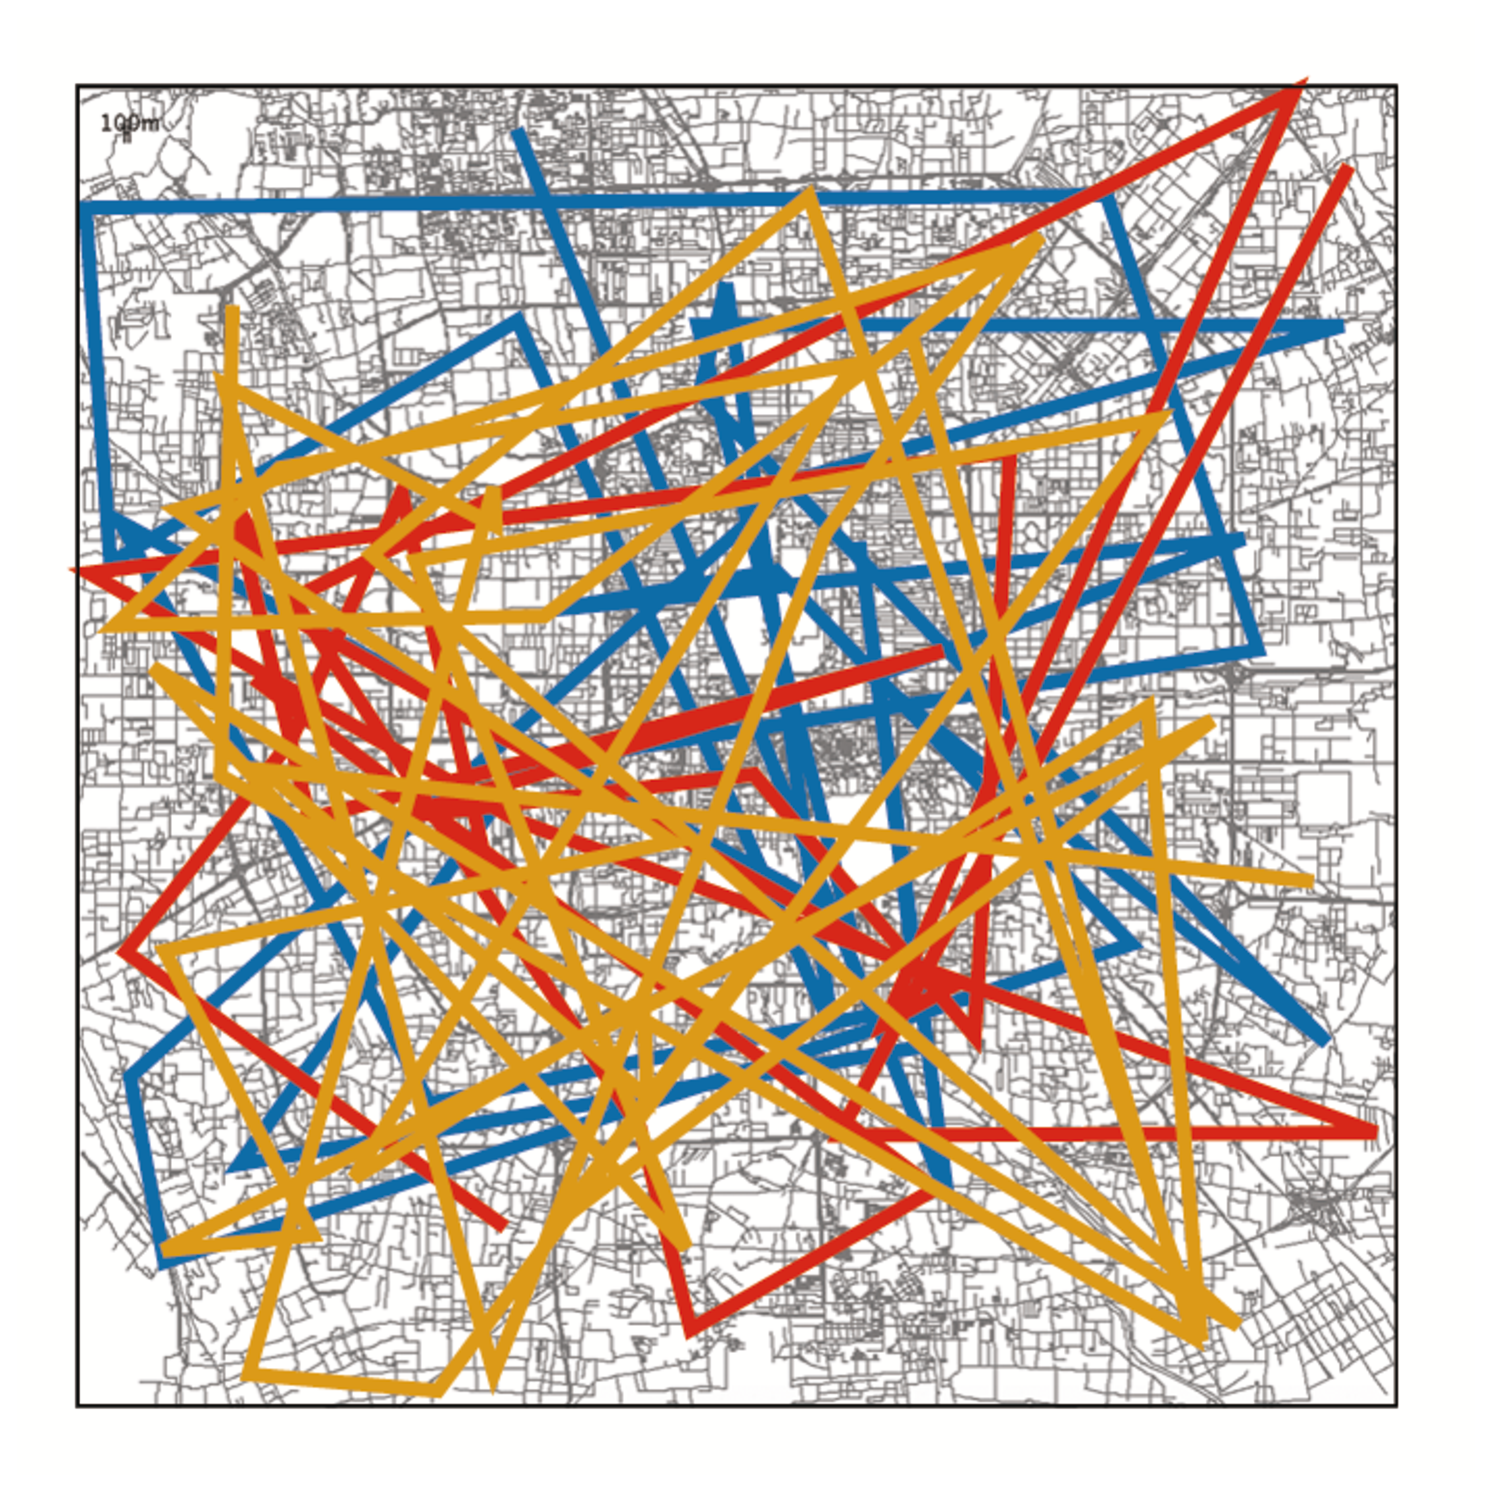
\includegraphics[width=0.24\textwidth]{figures/evalue/sample/rwp_traces.eps}}
\caption{Trace samples.}\label{figure_tracesample}
\end{figure}

\begin{figure}[!t]
\centering
\subfigure[Real Trace]{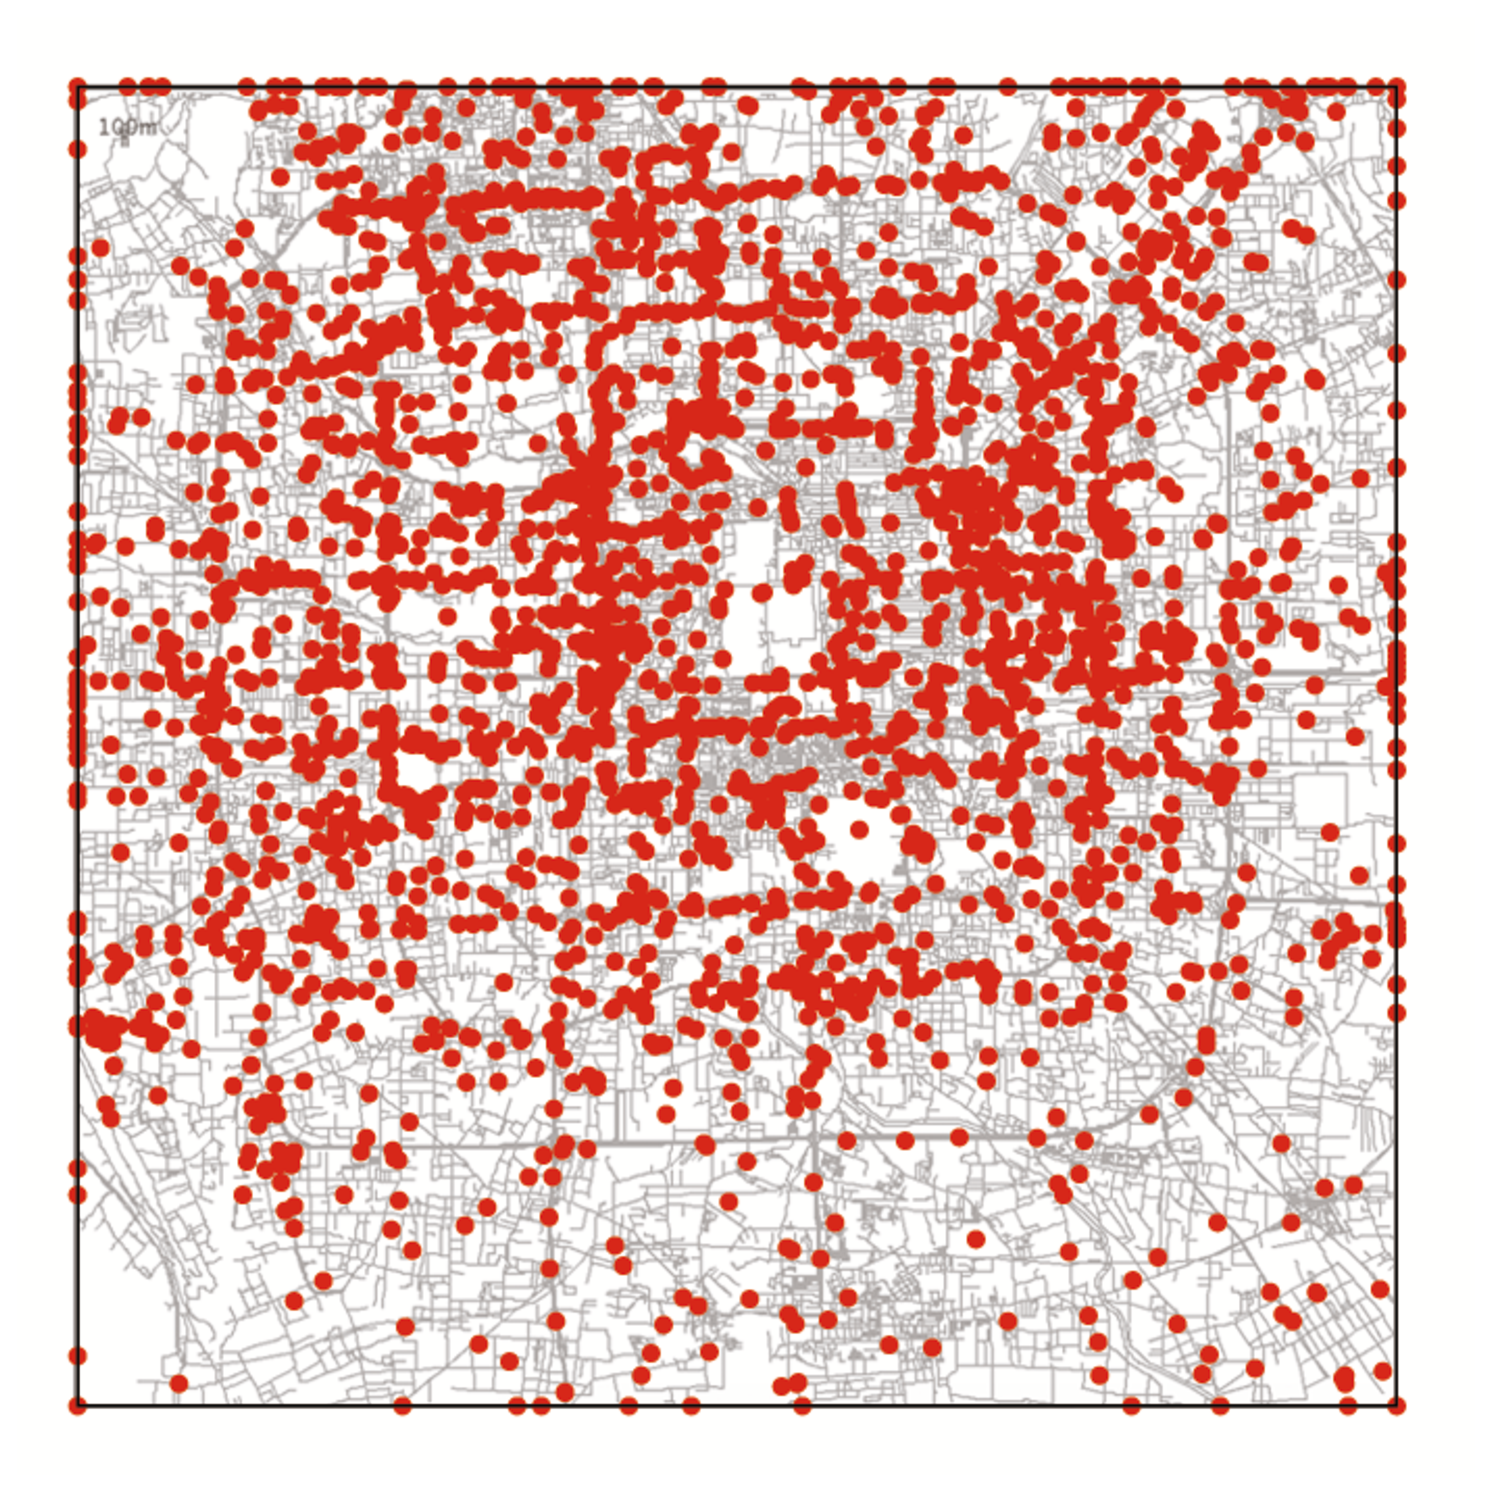
\includegraphics[width=0.24\textwidth]{figures/evalue/trace_nodedis.eps}}
\subfigure[T-START]{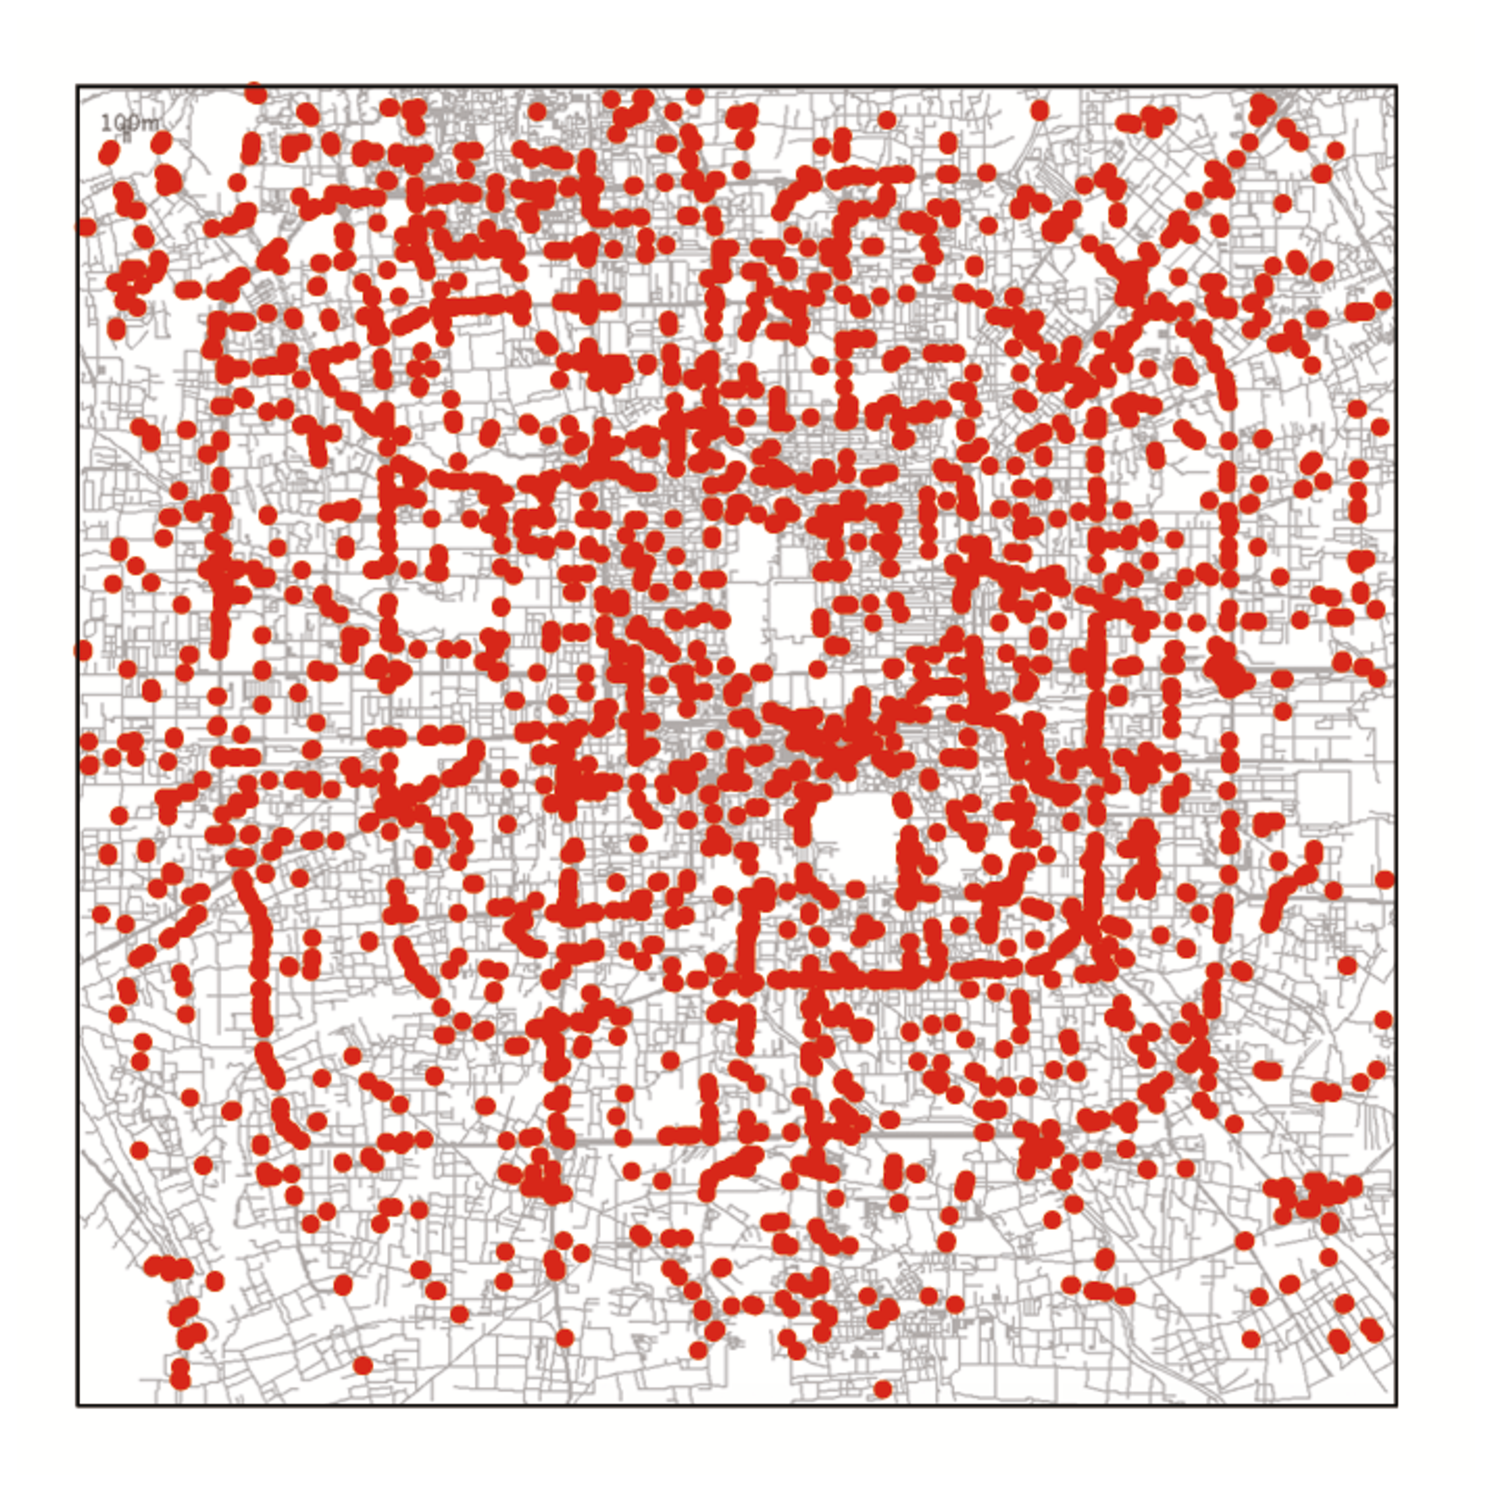
\includegraphics[width=0.24\textwidth]{figures/evalue/start_nodedis.eps}}
\subfigure[SP]{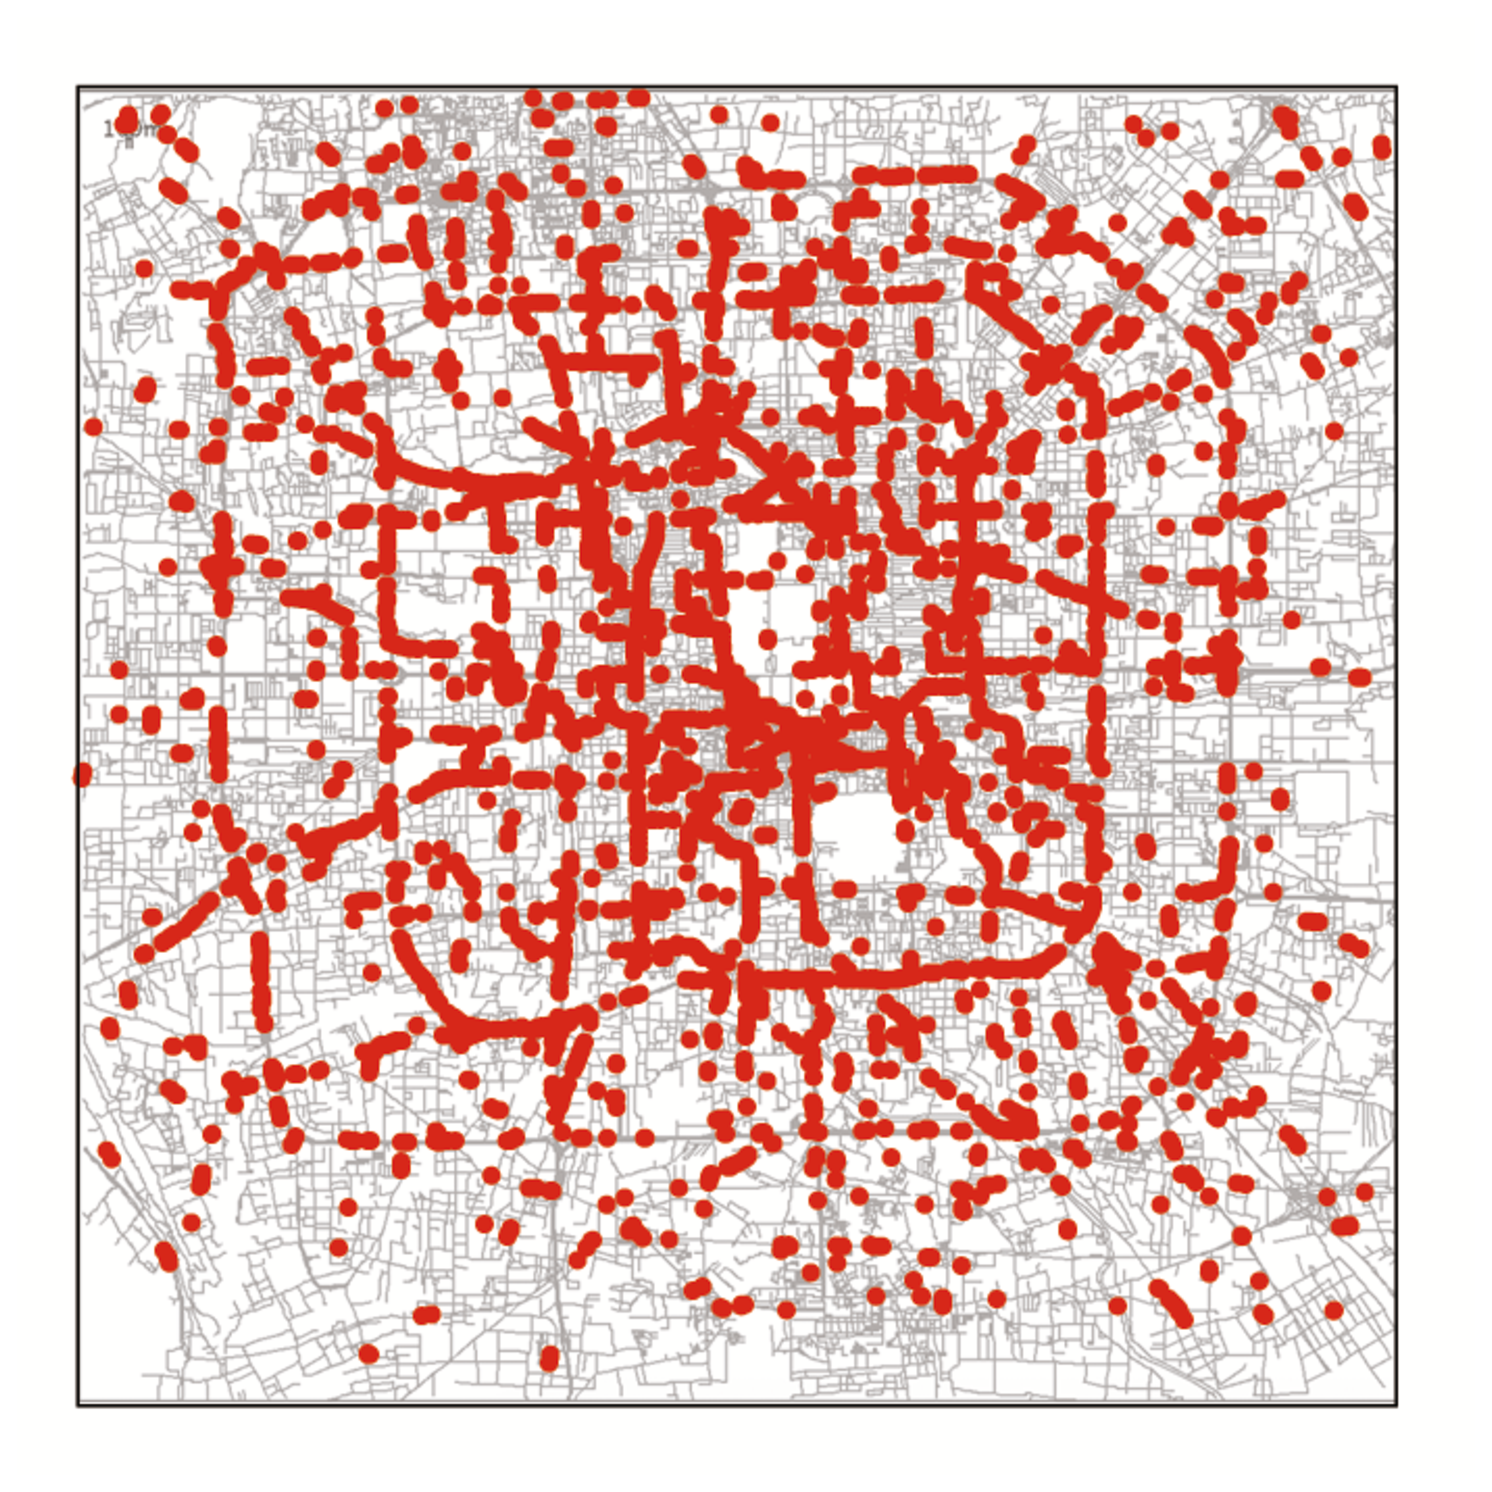
\includegraphics[width=0.24\textwidth]{figures/evalue/sp_nodedis.eps}}
\subfigure[RWP]{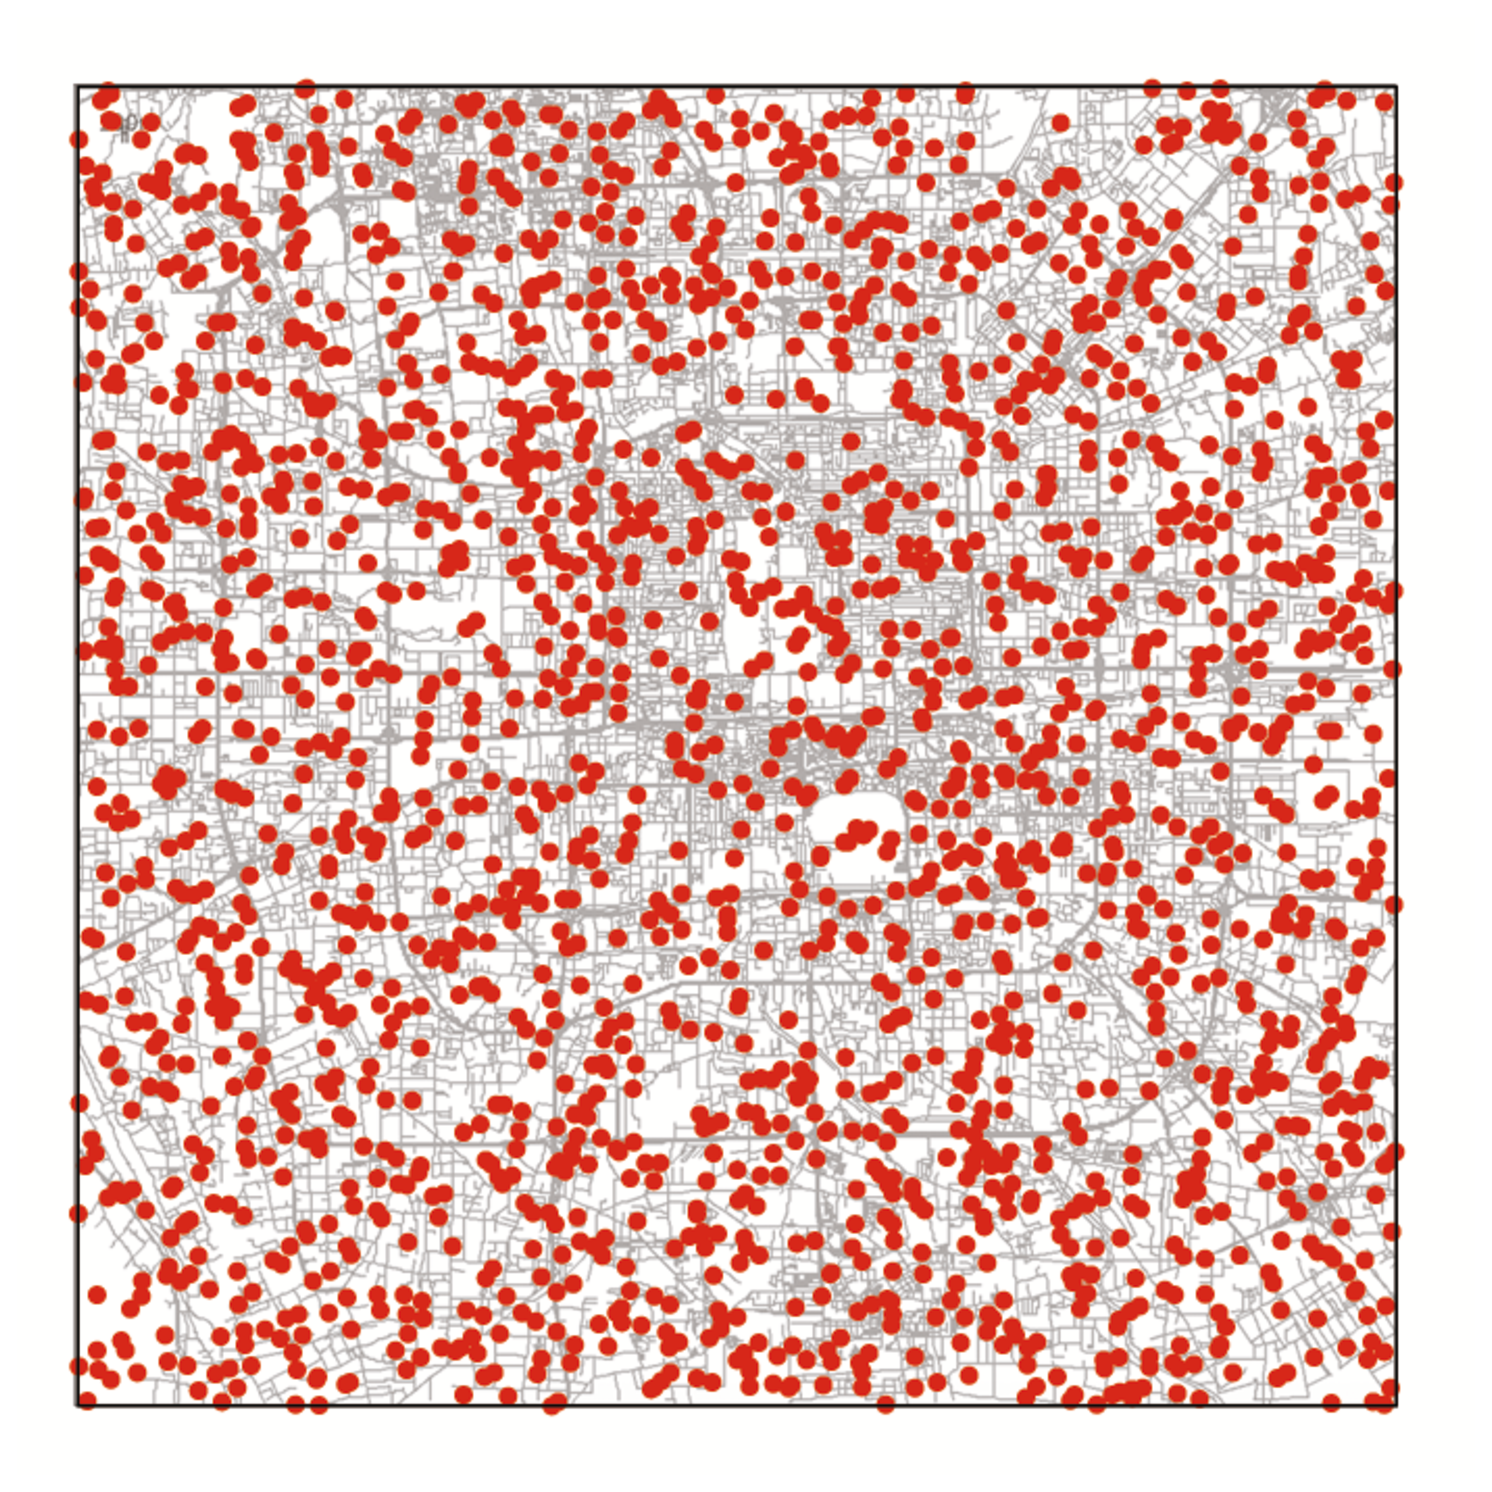
\includegraphics[width=0.24\textwidth]{figures/evalue/rwp_nodedis.eps}}
\caption{Nodes distribution snapshots.}\label{figure_trace_snapshots}
\end{figure}
Trace samples and their node distribution snapshots from different mobility models are reported in Fig.~\ref{figure_tracesample} and Fig~\ref{figure_trace_snapshots}. Fig.~\ref{figure_tracesample} shows the trace in one day. The traces of the real data and T-START only cover some parts of the area, while the traces of SP and RWP almost go through the whole area. Recall that SP and RWP select a destination randomly in the area, while T-START takes the associations between current region and destinations into consideration (which satisfies the movement rules of taxis). In Fig.~\ref{figure_trace_snapshots}, real trace, T-START and SP exhibit the road structures, while the node distribution of RWP is much uniform. As to T-START, the destination section process decides that it tends to select a destination in the regions with higher load/drop event probability. Therefore, with the decline of the randomness, the snapshot of T-START becomes much clear and centralized on the main roads, which matches real traces very well.
Since the node distribution has a great impact on the transport and network performance, a good understanding of it can help to route and control.  However, nodes are dynamic leading to a dynamic node distribution. In order to quantify the changing node distribution,  we introduce the in/out degree. The in/out degree figures out how many taxies moving in or out from a region in a time period. In/out degree defines how many nodes moveing in or out a area during a period of time. 
We divide the simulation scenario into grids of $ 400m \times 400 m$ to investigate the in/out degree, and the time period to measure the in/out degree is as two hours according to the simulation time. 
The average in-degree is equal to the average of out-degree. Because if a node moves out from area A to area B, the in-degree of B adds on one, meanwhile, the out-degree of area A adds on one. The average in/out degree are shown as table \ref{table_avg_inoutdegree}, and the variance of in-degree and out-degree are shown as table \ref{table_variance}.
We can figure out that the average in/out-degree for T-START and SP are similar with the Trace but that of RWP is relatively small. As to the variance of in/out-degree, from 6:00 to 8:00, the variance of T-START and SP are similar, however, the variance of T-START is larger than that of SP and more close to that of the real trace.  
\begin{figure}[!h]
\centering
\subfigure[average]{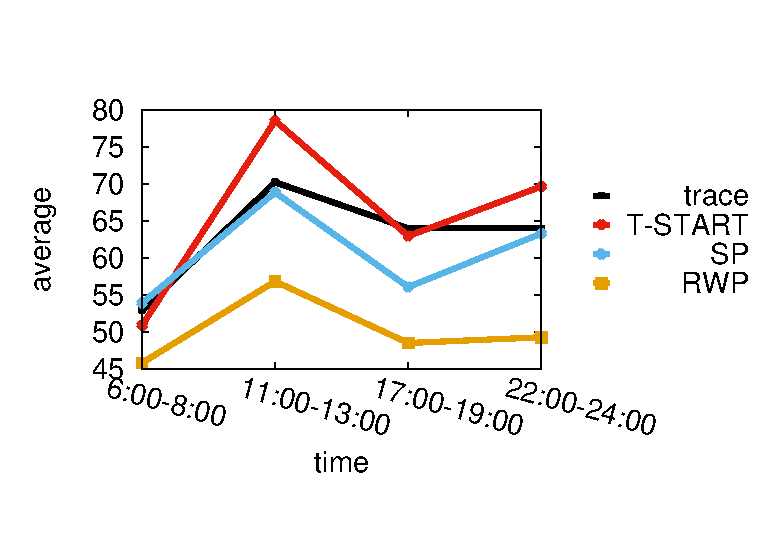
\includegraphics[width=0.5\textwidth]{figures/evalue/indegree/avg.eps}}
\subfigure[variance of in-degree]{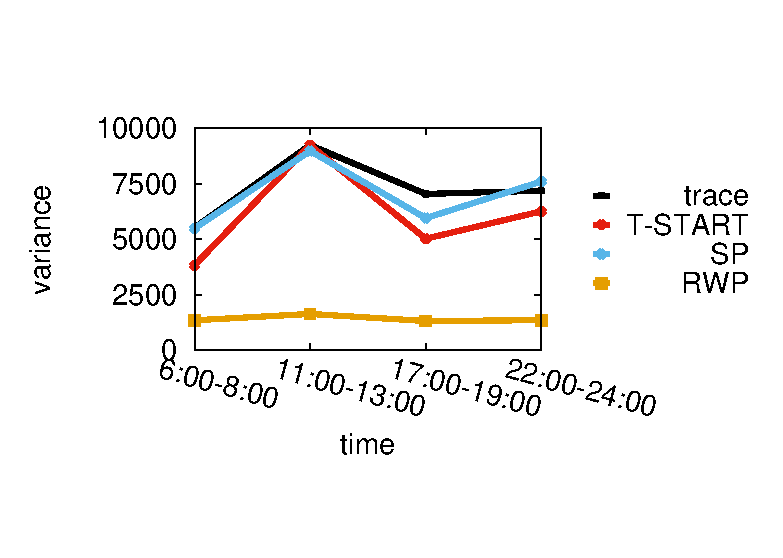
\includegraphics[width=0.5\textwidth]{figures/evalue/indegree/var_in.eps}}
\subfigure[variance of out-degree]{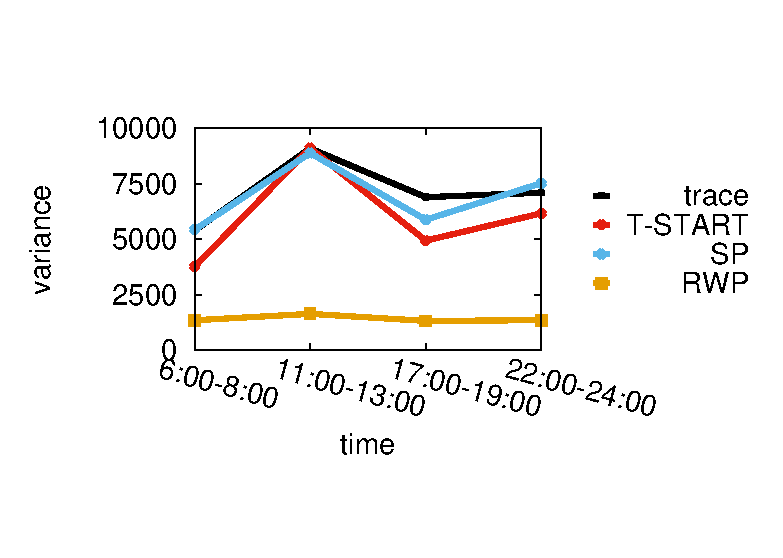
\includegraphics[width=0.5\textwidth]{figures/evalue/indegree/var_out.eps}}
\caption{average and variance of in/out-degree.}\label{figure_avg}
\end{figure}

\begin{table}[!h]
\caption{Average in/out-degree.}\label{table_avg_inoutdegree}
\centering
\begin{tabular}{r|c|c|c|c}
\hline
	&trace in Nov.8th	&T-START &SP &RWP\\
\hline
6:00-8:00&
52.899&50.868&53.909&45.797\\
11:00-13:00&
70.220&78.547&68.862&56.835\\  
17:00-19:00&
64.004&62.952&56.055&48.498\\
22:00-24:00&
63.993&69.644&63.301&49.271\\	
\hline
\end{tabular}
\end{table}

\begin{table}[!h]
\caption{Variance of the in/out-degree.}\label{table_variance}
\centering
\begin{tabular}{r|c|c|c|c}
\multicolumn{5}{c}{(a) in-degree}\\
\hline
	&trace of 8th	&T-START &SP &RWP\\
\hline
 6:00-8:00	&
5529.15&	3831.87&5501.827&	1357.65\\ 
 11:00-13:00&
9248.90&	9242.24&	8985.337&	1640.09\\
 17:00-19:00&
7049.92&	5030.80&	5958.505&	1324.26\\
 22:00-24:00&
7195.60&	6262.78&	7608.807&	1360.58\\
\hline
\end{tabular}
\begin{tabular}{r|c|c|c|c}
\hline
\multicolumn{5}{c}{(b) out-degree}\\
\hline
	&trace of 8th	&T-START &SP &RWP\\
\hline
 6:00-8:00	&
5,399.18&3,762.11&5436.401&1,358.32\\
 11:00-13:00&
9,097.05&9,115.16&8891.735&1,645.25\\
 17:00-19:00&
6,903.07&4,943.84&5884.668&1,329.40\\
 22:00-24:00&
7,102.49&6,175.93&7531.418&1,362.19\\
\hline
\end{tabular}
\end{table}
The in/out-degree distribution for the four time periods are ploted as figure \ref{figure_indegree_dis}.
For the RWP is similar, as figure \ref{figure_indegree_rwp}. We focus on the real trace, T-START and SP.  
From figure \ref{figure_indegree_dis}, the peaks of the real traces are contentrated on the main roads. For the T-START and SP use the Dijkstra algrothrithm, they will choose the shortest way to a destination, ignoring the factors of road condition. Nevertheless, we can find out some differences between T-START and SP. The peaks of indegree gather in the middle, because it chose the destination in a random way, while those of T-START distributes more to the ring roads.
\begin{figure}[h]
\centering
\epsfysize=2in\epsfbox{figures/evalue/indegree/17indegree_rwp.eps} 
\caption{The indegree distribtion for RWP from 17:00 to 19:00}\label{figure_indegree_rwp}
\end{figure}
\begin{figure}[h]
\centering
\begin{tabular}
[c]{ccc}
\epsfysize=1.2in\epsfbox{figures/evalue/indegree/6indegree_trace.eps} &
\epsfysize=1.2in\epsfbox{figures/evalue/indegree/6indegree_start.eps} &
\epsfysize=1.2in\epsfbox{figures/evalue/indegree/6indegree_sp.eps} \\
\epsfysize=1.2in\epsfbox{figures/evalue/indegree/11indegree_trace.eps} &
\epsfysize=1.2in\epsfbox{figures/evalue/indegree/11indegree_start.eps} &
\epsfysize=1.2in\epsfbox{figures/evalue/indegree/11indegree_sp.eps} \\
\epsfysize=1.2in\epsfbox{figures/evalue/indegree/17indegree_trace.eps} &
\epsfysize=1.2in\epsfbox{figures/evalue/indegree/17indegree_start.eps} &
\epsfysize=1.2in\epsfbox{figures/evalue/indegree/17indegree_sp.eps} \\
\epsfysize=1.2in\epsfbox{figures/evalue/indegree/22indegree_trace.eps} &
\epsfysize=1.2in\epsfbox{figures/evalue/indegree/22indegree_start.eps} &
\epsfysize=1.2in\epsfbox{figures/evalue/indegree/22indegree_sp.eps} \\
(a) Traces of Nov.8th & (b) T-START & (c) SP \\
\end{tabular}
\caption{The indegree distribtion for the real trace, T-START and SP}\label{figure_indegree_dis}
\end{figure}
In order to quantity the similarity between the mobility models and the real traces, we introduce the conception of the relative error. 
The relative error is calculated as:
\begin{equation}
    \delta = \frac{\sum \Delta x}{\sum x_{real}} 
\end{equation}
$\Delta x$ is the absolute value of the compare value minus the real one, and $x_{real}$ is the real value.

Firstly, in order to find out the relative error is valid, we extracted the in/out-degree matrixes from November 1 to November 7 for the four time periods, and then obtain a average matrix for every time period. Then, we compare the in/out-degree of every single day of the seven days with the average matrix, the results are shown as table \ref{table_relative_err_avg}. The relative error between every day with corresponding matrix are in a range from 0.1 to 0.25. It shows that the in/out-degree distributions for different time periods have certain regularity and we can utilize the average matrix for corresponding time as a comparition. 
\begin{table}[!t]
\centering
\caption{The relative error compared with the average for in-degree and out-degree}\label{table_relative_err_avg}
\begin{tabular}[c]{c|c|c|c|c|c|c|c}
\multicolumn{8}{c}{(a) in-degree}\\
\hline
item& 1th&2th&3th&4th&5th&6th&7th\\
\hline
6:00-8:00&
0.1139& 
0.1485&
0.1732&
0.1372&
0.1500&
0.2489&
0.1507\\
11:00-13:00&
0.1056&
0.0953&
0.1509&
0.0994&
0.1714&
0.1294&
0.1011\\
17:00-19:00&
0.1537&
0.1728&
0.1491&
0.1888&
0.1338&
0.1303&
0.1407\\
22:00-24:00&
0.1360&
0.1054&
0.1637&
0.1183&
0.1467&
0.1470&
0.1076\\
\hline
\end{tabular}
\begin{tabular}[c]{c|c|c|c|c|c|c|c}
\multicolumn{8}{c}{(b) out-degree}\\
\hline
item& 1th&2th&3th&4th&5th&6th&7th\\
\hline
6:00-8:00&
0.1132&
0.1481&
0.1726&
0.1374&
0.1499&
0.2478&
0.1507\\
11:00-13:00&
0.1057&
0.0953&
0.1509&
0.0998&
0.1719&
0.1296&
0.1012\\
17:00-19:00&
0.1534&
0.1725&
0.1488&
0.1890&
0.1336&
0.1298&
0.1412\\
22:00-24:00&
0.1358&
0.1057&
0.1636&
0.1184&
0.1468&
0.1469&
0.1075\\
\hline
\end{tabular}
\end{table}
Therefore, compare of the average in/out-degree matrix, the relative errors of the trace of Nov.8th, T-START, SP and RWP are shown as table \ref{table_relative_err}.
The relative error of the trace of Nov.8th remains in a low level about 0.1.
The relative error of T-START is about 0.48, while that of SP is about 0.65 and RWP is more than 0.8 for every time period.  
\begin{table}[!h]
\caption{The relative error.}\label{table_relative_err}
\centering
\begin{tabular}{r|c|c|c|c}
\hline
	&trace of 8th	&T-START &SP &RWP\\
\hline
 6:00-8:00&
0.1278&	0.4927&	0.6923&	0.8037\\ 
 11:00-13:00&
0.1051&	0.4888&	0.6783&	0.8360\\
 17:00-19:00&
0.1161&	0.4694&	0.6533&	0.8382\\
 22:00-24:00&
0.1276&	0.4812&	0.6840&	0.8177\\
\hline
\end{tabular}
\begin{tabular}{r|c|c|c|c}
\hline
	&trace of 8th	&T-START &SP&RWP\\
\hline
 6:00-8:00&
0.1279&	0.4952&	0.6903&	0.8030\\
 11:00-13:00&
0.1055&	0.4908&	0.6766&	0.8371\\
 17:00-19:00&
0.1160&	0.4730&	0.6515&	0.8380\\
 22:00-24:00&
0.1276&	0.4842&	0.6821&	0.8179\\
\hline
\end{tabular}
\end{table}
\begin{figure}[h]
\centering
\subfigure[relative error of in-degree]{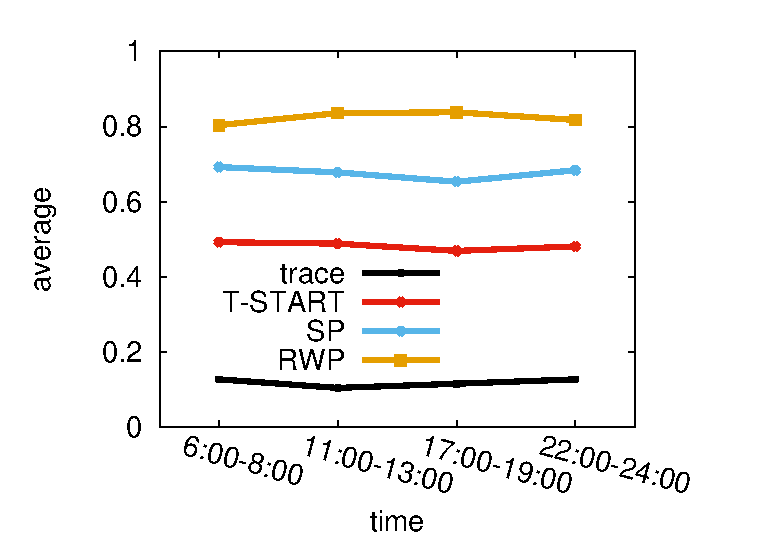
\includegraphics[width=0.45\textwidth]{figures/evalue/indegree/err_in.eps}}
\subfigure[relative error of out-degree]{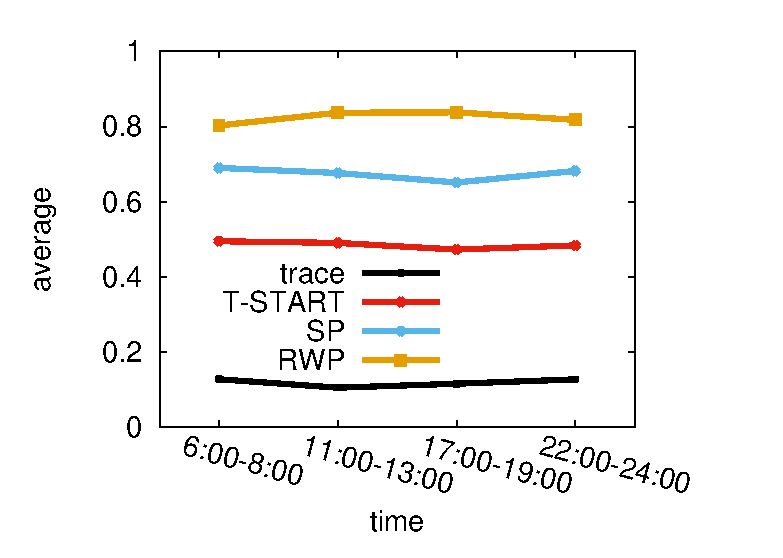
\includegraphics[width=0.45\textwidth]{figures/evalue/indegree/err_out.eps}}
\caption{average and variance of in/out-degree.}\label{figure_avg}
\end{figure}
